\section{Exercises on Minimum Spanning Trees Problems}

	\paragraph{}
\begin{quote}
	GTC has been provided with 50 locations to connect in a certain country. These locations need
to be connected in such a way that any two of these locations are able to communicate
with each other. All the connections need not be direct. Due to high bandwidth
requirements, GTC will use high capacity cables for the connections, and wants to
know the costs of laying the cable under various circumstances. In Figure \ref{graph2-1} we
have schematically depicted the 50 locations and all possible direct connections. The
numbers attached to the connections in Figure \ref{graph2-1} refer to the distances (in 10 kilometer
units) between locations. The cost of the cable is \texteuro 5,000 per kilometer.
\end{quote}

\begin{figure}[H]
	\centering
	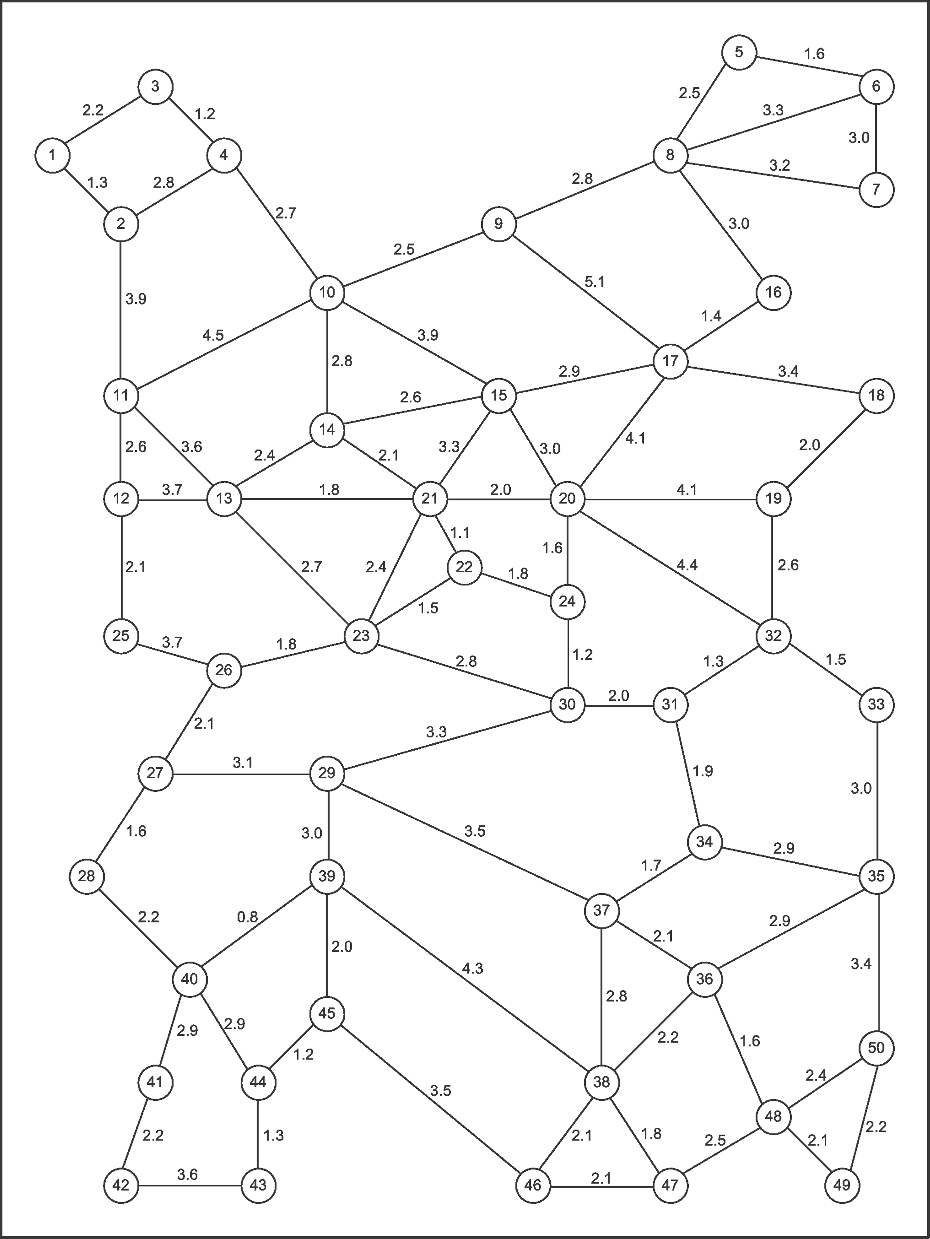
\includegraphics[scale=0.5]{./img/graph2-1.png}
	\caption{Schematic map with 50 locations (distances in 10 kilometer units, costs in \texteuro5,000per kilometer)}
	\label{graph2-1}
\end{figure}

\subsection{Problem 2.1. Reliable Cable Connections}
\begin{enumerate}[(a)]
\item \begin{quote}Calculate the minimum length of cable needed to connect all locations in Figure
\ref{graph2-1}. Also give the list of connections that are used for the cabling.\end{quote}

	\paragraph{}
	Let's consider a graph with vertices corresponding to the locations in a country and edges corresponding to possible direct connections. This graph is undirected because the cable connections transmit data in both directions and weighted --- weight of a particular edge connecting two vertices is a length of a possible direct connection in km between two corresponding locations.

	\paragraph{}
	Then the sought for system of connections between locations with a minimum length of cable required is a minimum spanning tree in a described graph. Indeed in the spanning tree there is a unique path between each pair of vertices so there are no redundant connections and every location is able to communicate with other locations using cables of this system. Also by definition the sum of weights of edges in a MST is minimal possible among all the spanning trees of the graph so this system requires the minimal possible length of cable to connect all the locations thus the minimal possible sum of money because we pay equally \texteuro 5,000 for every km.

	\paragraph{}
	MST problem can be solved efficiently using Kruskal's algorithm. The edges of the MST (the connections between locations in the country) are listed in figure \ref{mst2-1-a}. The length of cable needed to connect all locations is 1000 km which results in a \texteuro 5,000,000 total price of the system.

\begin{figure}[H]
	\centering
	\begin{multicols}{5}
(1,~2), (1,~3), (3,~4), (4,~10), (5,~6), (5,~8), (6,~7), (8,~9), (9,~10), (10,~14), (11,~12), (11,~13), (12,~25), (13,~21), (14,~15), (14,~21), (15,~17), (16,~17), (18,~19), (19,~32), (20,~24), (21,~22), (22,~23), (22,~24), (23,~26), (24,~30), (26,~27), (27,~28), (28,~40), (29,~39), (30,~31), (31,~32), (31,~34), (32,~33), (34,~35), (34,~37), (36,~37), (36,~38), (36,~48), (38,~46), (38,~47), (39,~40), (39,~45), (40,~41), (41,~42), (43,~44), (44,~45), (48,~49), (49,~50)
	\end{multicols}
	\caption{List of connections in a minimum cost communication system}
	\label{mst2-1-a}
\end{figure}

\item \begin{quote}GTC regrets that the locations 9 and 17 are not directly connected in the solution
of part (a). There can be taken two ways to get 9 and 17 connected --- adding
a direct cable between 9 and 17 to the solution of Problem 2.1(a) and deleting a
most expensive connection in the cycle thus created, or repeating the calculations
of Problem 2.1(a) with the extra restriction that the connection 9~--~17 has to be
in the new solution. Compare both methods. Will both methods always give the
same result? Explain your answer.\end{quote}

	\paragraph{}
	Both methods will always give the same result. The 9~--~17 edge will produce a cycle 9~--~10~--~14~--~15~--~17~--~9 where the heaviest edge besides 9~--~17 is 15~--~17 that will be removed from the tree. The resulting tree will have a total cable length of 1022 km with a total cost of \texteuro 5,110,000.

	\paragraph{}
	The equivalence of both methods can be easily shown if one follows the steps of the Kruskal's algorithm. According to the Kruskal's algorithm the MST is built incrementally edge by edge in the ascending order of weights. The important part is that on each iteration of the algorithm the current edge is either added to the MST or disregarded since it produces a cycle. So if an edge was once added to MST than it wouldn't be deleted later. Thus we can consider the iterative consecutive process of building cycle 9~--~10~--~14~--~15~--~17~--~9 edge by edge instead of adding 9~--~17 to the complete MST. Since the algorithm iterates through edges in the ascending order of weights the last two edges to consider will be 15~--~17 and 9~--~17 as the heaviest ones. But one can make these two edges equally suitable for the Kruskal algorithm by increasing the weight of 15~--~17 to match the weight of 9~--~17. After that the algorithm can naturally pick the edge 9~--~17 thus building a new spanning tree with total weight increased by exactly the weight difference of edges 9~--~17 and 15~--~17. But increasing the weight of 15~--~17 is the exact equivalence of adding 9~--~17 to spanning tree as the first edge from this cycle since the Kruskal's algorithm will add the remaining edges in ascending order of weight thus leaving the 15~--~17 behind as the second heaviest.

\item \begin{quote}The cable system designed in part (a) is not very reliable, in the sense that there
is only one connection between any pair of locations. Why is this so?
Determine, by inspection, a most vulnerable connection in your solution to part
(a), in the sense that if the cable on this connection breaks down, the most number
of pairs of locations will not be able communicate anymore.\end{quote}

	\paragraph{}
	The cable system designed in part (a) is not very reliable because the cable connections form a tree. As a result there is a unique path between every pair of vertices. Thus the removal of any edge will cause the graph to lose connectivity.

	\paragraph{}
	The ``vulnerability'' of the direct connection in the described sense can be calculated in a single traverse of a tree using DFS. Starting the DFS naturally roots the tree thus it's becomes easy to calculate the answer for the edge by computing the size of the subtree of the deeper vertex of the edge. The size of the other subtree (to the other part of the edge) is computed as a difference between the total number of vertices and the size of the first subtree. The sought for ``vulnerability'' is a product of sizes of these subtrees.

	\paragraph{}
	The most vulnerable connection is 21~--~22. The break down of this connection will cause 589 pairs of locations (31 on the one side of the edge and 19 on another) to lose contact with each other.

\item \begin{quote}Design a reliable cable connection, in the sense that if the cable between any
two locations breaks down, there is still a connection (although possibly indirect)
between these locations. Is your design the cheapest possible?\end{quote}

	\paragraph{}
	The cable system will be reliable in a described sense if it's corresponding graph has no bridges~--- is 2-edge-connected. It is known that the problem of finding minimum spanning subgraphs with these property is NP-hard \cite{garey79}. Since it's hard to find the optimal solution~--- minimum spanning 2-edge-connected subgraph, we will compute the minimal spanning 2-edge-connected subgraph (a removal of any edge in such subgraph leads to lose of 2-edge-connectivity). For this task the simple $O(m(n+m))$ ($n$~--- number of vertices, $m$~--- number of edges) algorithm is suitable~--- we try to delete each edge from the graph and if after the removal the 2-edge-connectivity is preserved than we delete this edge permanently. Else we add this edge to the resulting spanning subgraph. The edges of this subgraph are listed in figure \ref{reliable1}. The cable length of the system equals 1373 km with a total cost of \texteuro 6,865,000.

\begin{figure}[H]
	\centering
	\begin{multicols}{5}
(1,~2), (1,~3), (2,~11), (3,~4), (4,~10), (5,~6), (5,~8), (6,~7), (7,~8), (8,~9), (8,~16), (9,~10), (11,~12), (11,~13), (12,~25), (13,~14), (14,~15), (15,~17), (16,~17), (17,~18), (18,~19), (19,~20), (19,~32), (20,~21), (21,~23), (22,~23), (22,~24), (23,~26), (24,~30), (25,~26), (27,~28), (27,~29), (28,~40), (29,~30), (29,~37), (30,~31), (31,~32), (32,~33), (33,~35), (34,~35), (34,~37), (35,~36), (35,~50), (36,~38), (38,~39), (39,~40), (40,~41), (41,~42), (42,~43), (43,~44), (44,~45), (45,~46), (46,~47), (47,~48), (48,~49), (49,~50)
	\end{multicols}
	\caption{List of connections in a reliable communication system}
	\label{reliable1}
\end{figure}

\end{enumerate}

\subsection{Problem 2.2. What Happens If}
\begin{quote}In another country, GTC can obtain the rights to construct a main cable network that
will connect the 46 major towns of this country. The country is very mountainous
and a number of large lakes and rivers makes the construction of the cable network
very delicate for the environment. These regions are called ``vulnerable'' and no industrial
activity is normally allowed in these regions. Therefore, if GTC lays cable in
vulnerable regions, it has to pay the government a certain amount of money, called
``environmental price'' for environmental restoration activities. In Figure \ref{graph2-2} the 46
cities are schematically depicted. Attached to the regions (connections between the
cities) are the costs of laying the cable (first number) plus the environmental price
GTC has to pay to the government (second number).\end{quote}

\begin{figure}[H]
	\centering
	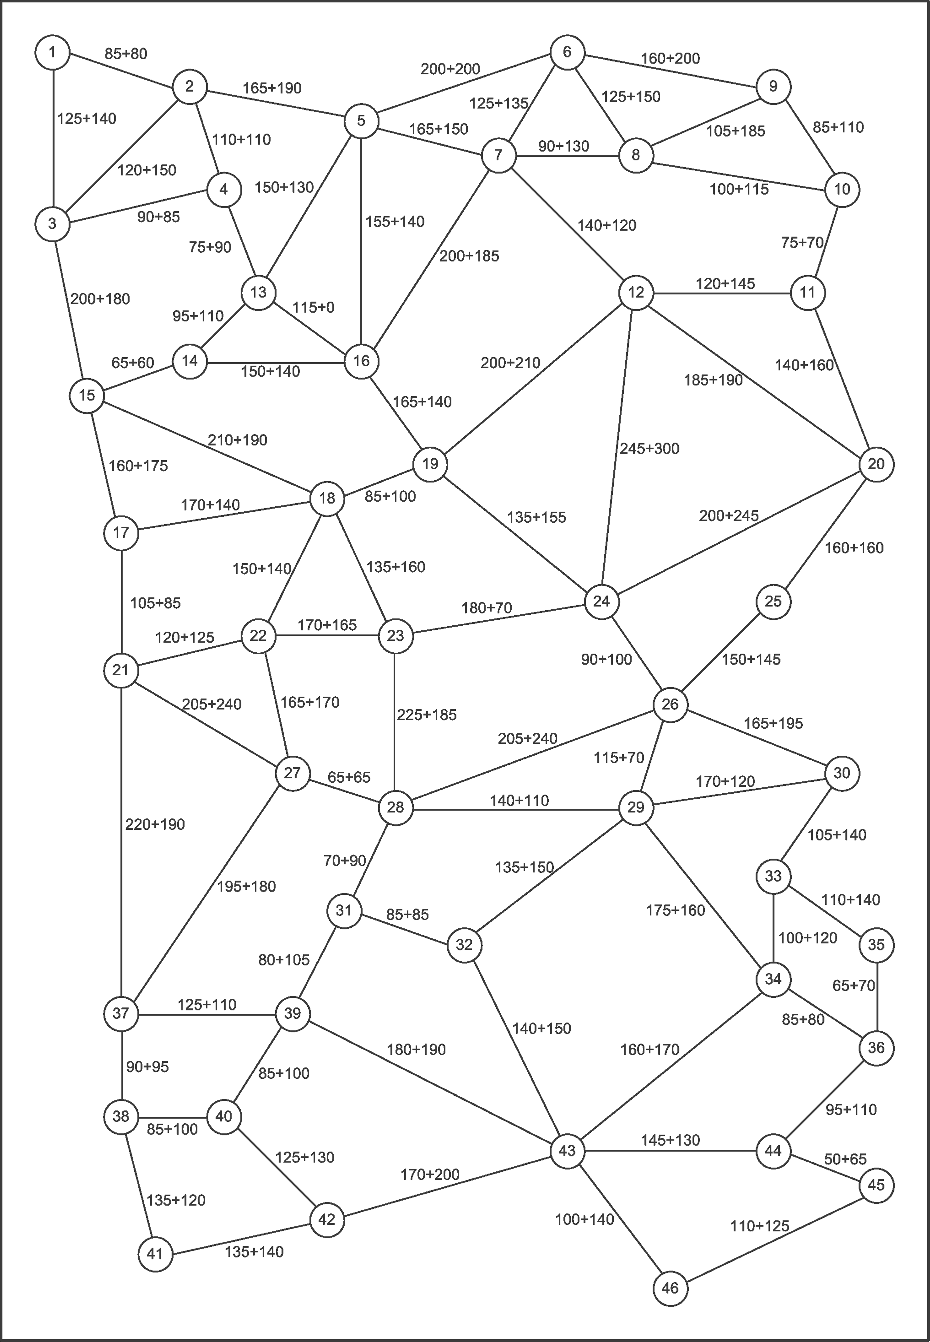
\includegraphics[scale=0.5]{./img/graph2-2.png}
	\caption{Schematic road map with 46 locations (connection cost = cable cost + environmental cost, costs in \texteuro 1,000)}
	\label{graph2-2}
\end{figure}

\begin{enumerate}[(a)]
\item \begin{quote}Is it possible to lay the cables in such a way that each pair of cities are connected
and the total cost does not exceed \texteuro 9,500,000?\end{quote}

	\paragraph{}
	Let's consider a graph with vertices corresponding to the locations in a country and edges corresponding to possible direct connections. This graph is undirected because the cable connections transmit data in both directions and weighted --- weight of a particular edge connecting two vertices is a sum of cable cost and environmental cost of the direct connection.

	\paragraph{}
	Then the sought for minimum cost system of connections between locations is a minimum spanning tree in a described graph. Indeed in the spanning tree there is a unique path between each pair of vertices so there are no redundant connections and every location is able to communicate with other locations using cables of this system. Also by definition the sum of weights of edges in a MST is minimal possible among all the spanning trees of the graph so this system requires the minimal possible cost to connect all the locations.

	\paragraph{}
	MST problem can be solved efficiently using Kruskal's algorithm. The edges of the MST (the connections between locations in the country) are listed in figure \ref{mst2-2-a}. The minimum cost of a network needed to connect all locations is \texteuro 9,595,000 which is greater than required \texteuro 9,500,000.

\begin{figure}[H]
	\centering
	\begin{multicols}{5}
(1,~2), (2,~4), (3,~4), (4,~13), (5,~7), (5,~13), (6,~7), (7,~8), (7,~12), (8,~10), (9,~10), (10,~11), (11,~20), (13,~14), (13,~16), (14,~15), (16,~19), (17,~21), (18,~19), (18,~22), (19,~24), (21,~22), (23,~24), (24,~26), (25,~26), (26,~29), (27,~28), (28,~29), (28,~31), (29,~30), (30,~33), (31,~32), (31,~39), (33,~34), (34,~36), (35,~36), (36,~44), (37,~38), (38,~40), (38,~41), (39,~40), (40,~42), (43,~46), (44,~45), (45,~46)
	\end{multicols}
	\caption{List of connections in a minimum cost cable network}
	\label{mst2-2-a}
\end{figure}

\item \begin{quote}Since the cabling project is important for the country, the government is open to
negotiating with GTC on regions where the environmental price could be lowered.
In case the answer to part (a) is ``no'', then choose a number of regions on
which GTC should start negotiations with the government.
GTC realizes that the government is willing to lower the prices by a maximum of
15\% in five regions. Is there a cable system that satisfies the budget of the company
and the margins of the government? At what percentage reduction would
such a project just be feasible?\end{quote}

	\paragraph{}
	Since the number of edges to be discounted is rather small we can check all the possible sets of 5 edges and apply discount to them. After applying discount we build MST and among all MSTs we choose the one with the minimum total weight. After checking all the possible variants we obtain that in order to get the maximal profit we should apply discount to connections (32,~43), (25,~26), (19,~24), (11,~20) and (5,~7). The edges of the resulting tree are listed in figure \ref{mst2-2-b}. The total cost equals \texteuro 9,481,000 which is less than required \texteuro 9,500,000.

\begin{figure}[H]
	\centering
	\begin{multicols}{5}
(1,~2), (2,~4), (3,~4), (4,~13), (5,~7), (5,~13), (6,~7), (7,~8), (7,~12), (8,~10), (9,~10), (10,~11), (11,~20), (13,~14), (13,~16), (14,~15), (16,~19), (17,~21), (18,~19), (18,~22), (19,~24), (21,~22), (23,~24), (24,~26), (25,~26), (26,~29), (27,~28), (28,~29), (28,~31), (30,~33), (31,~32), (31,~39), (32,~43), (33,~34), (34,~36), (35,~36), (36,~44), (37,~38), (38,~40), (38,~41), (39,~40), (40,~42), (43,~46), (44,~45), (45,~46)
	\end{multicols}
	\caption{List of connections in a minimum cost cable network after applying 15\% discount to 5 connections}
	\label{mst2-2-b}
\end{figure}

	\paragraph{}
	The minimal discount that makes the project feasible can be calculated by applying binary search on a discount value. The sought for discount equals $\approx$12.5\%.

\item \begin{quote}Actually, the price of traversing the region between the cities 5 and 13 could not
be determined with the same accuracy as the other prices. How much can the
price of intersecting the region between 5 and 13 change before a different cable
network is more profitable for GTC?\end{quote}

	\paragraph{}
	Edge (5,~13) is present in the MST, so the answer for this question is the upper tolerance value for this edge. By definition it's a maximal increase in weight that leaves this edge in the MST. The upper tolerance equals the weight difference between  the MST built ignoring edge (5,~13) and the original MST or equivalently the upper tolerance equal the weight difference of the first edge that creates the cycle in MST which includes edge (5,~13) when calculating the MST with the Kruskal's algorithm and the edge (5,~13), since adding exactly that value to the weight of an edge will make another equally suitable for the Kruskal's algorithm. The edge that could replace (5,~13) in the MST after increasing the weight of (5,~13) by it's upper tolerance is (5,~16), so the upper tolerance of (5,~13) equals \texteuro 15,000.

\item \begin{quote}After a consultation round with all people and organizations involved, it is decided
that the links 6~--~9 and 15~--~17 have to be included in the new cable
network, whereas the links 24~--~26 and 31~--~39 will not be included. Determine
a minimal cost solution, without the reductions.
The government was willing to lower the price for the edges 6~--~9 and 15~--~17
by 10\% on top of the negotiations from part (b). Was this 10\% enough for the
project to be financially feasible?\end{quote}

	\paragraph{}
	To find the required cable network system we force edges (6,~9), (15,~17) to be in the MST in the beginning of the Kruskal's algorithm and ignore edges (24,~26) and (31,~39) when building the MST. The edges of the minimum cost solution satisfying these requirements are listed in Figure \ref{mst2-2-d-1}. The total cost of this network is \texteuro 10,040,000 which is far from being financially feasible.

\begin{figure}[H]
	\centering
	\begin{multicols}{5}
(1,~2), (2,~4), (3,~4), (4,~13), (5,~7), (5,~13), (6,~9), (7,~8), (7,~12), (8,~10), (9,~10), (10,~11), (11,~20), (13,~14), (13,~16), (14,~15), (15,~17), (17,~21), (18,~19), (18,~22), (19,~24), (20,~25), (21,~22), (23,~24), (25,~26), (26,~29), (27,~28), (28,~29), (28,~31), (29,~30), (30,~33), (31,~32), (33,~34), (34,~36), (35,~36), (36,~44), (37,~38), (38,~40), (38,~41), (39,~40), (39,~43), (40,~42), (43,~46), (44,~45), (45,~46)
	\end{multicols}
	\caption{List of connections in a minimum cost cable network with connections (6,~9) and (15,~17) forced to be in the solution and connections (24,~26) and (31,~39) ignored}
	\label{mst2-2-d-1}
\end{figure}

	\paragraph{}
	Now let's lower the environmental cost of connections (6,~9) and (15,~17) by 10\% and apply the algorithm from part (b) of using the most out of 15\% discount on 5 connections. The edges of the minimum cost solution are listed in figure \ref{mst2-2-d-2}. Even after applying both 10\% discounts for edges (6,~9) and (15,~17) and 15\% discount for edges (42,~43), (20,~25), (19,~24), (11,~20), (5,~7) the total cost of the solution is \texteuro 9,878,750 which is clearly financially unfeasible.

\begin{figure}[H]
	\centering
	\begin{multicols}{5}
(1,~2), (2,~4), (3,~4), (4,~13), (5,~7), (5,~13), (6,~9), (7,~8), (7,~12), (8,~10), (9,~10), (10,~11), (11,~20), (13,~14), (13,~16), (14,~15), (15,~17), (17,~21), (18,~19), (18,~22), (19,~24), (20,~25), (21,~22), (23,~24), (25,~26), (26,~29), (27,~28), (28,~29), (28,~31), (29,~30), (30,~33), (31,~32), (33,~34), (34,~36), (35,~36), (36,~44), (37,~38), (38,~40), (38,~41), (39,~40), (40,~42), (42,~43), (43,~46), (44,~45), (45,~46)
	\end{multicols}
	\caption{List of connections in a minimum cost cable network with connections (6,~9) and (15,~17) forced to be in the solution and connections (24,~26) and (31,~39) ignored with all the discounts applied}
	\label{mst2-2-d-2}
\end{figure}

\end{enumerate}

\subsection{Problem 2.6. Designing a Radio Telescope}
\begin{quote}
The astronomical society ASTRO wants to build a large radio telescope. The telescope
will consist of thirteen sensors laid out in a four armed spiral in the countryside.
Figure \ref{map2-6} shows the location of the sensors marked A, B, . . . , M. Each of
these sensors continuously collect vast amounts of data, and these data need to be
sent to a central processing station located at A for analysis. GTC has been asked to
provide the physical connection to make this data transfer possible. The cable connections
that ASTRO requires need to be reliable, and so the cost of laying cable is
quite high, about \texteuro 10 per meter of cable laid.
\end{quote}

\begin{figure}[H]
	\centering
	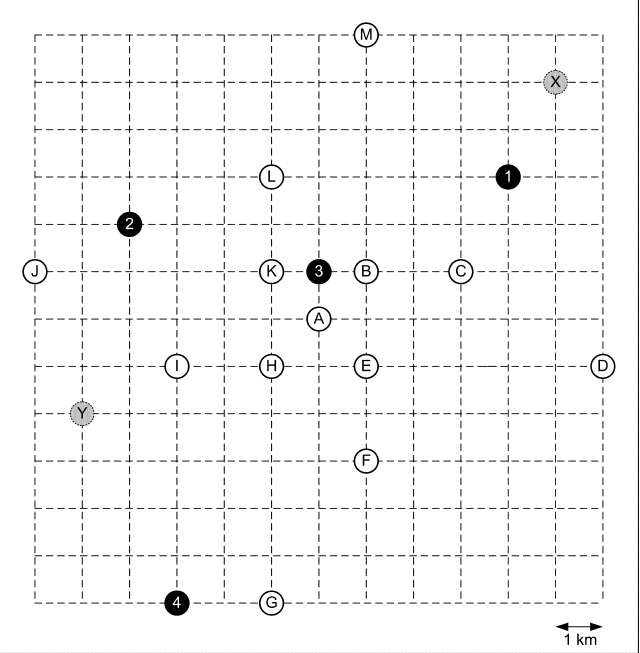
\includegraphics[scale=0.5]{./img/map2-6.png}
	\caption{Schematic map of the telescope sensors, the access points, and the cities}
	\label{map2-6}
\end{figure}

\begin{enumerate}[(a)]
\item \begin{quote}What is GTC’s minimum investment in cable laying in order to complete the
project?\end{quote}

	\paragraph{}
	Let's consider a graph with vertices corresponding to the locations of sensors and edges corresponding to possible direct connections between these sensors. This graph is undirected because the cable connections transmit data in both directions and weighted --- weight of a particular edge connecting two vertices is a Euclidean distance in km between two corresponding locations.

	\paragraph{}
	Then the sought for system of connections between locations with a minimum length of cable required is a minimum spanning tree in a described graph. Indeed in the spanning tree there is a unique path between each pair of vertices so there are no redundant connections and every location is able to communicate with other locations using cables of this system. Also by definition the sum of weights of edges in a MST is minimal possible among all the spanning trees of the graph so this system requires the minimal possible length of cable to connect all the locations thus the minimal possible sum of money because we pay equally \texteuro 10 for every m or \texteuro 10,000 per km.

	\paragraph{}
	MST problem can be solved efficiently using Kruskal's algorithm. The edges of the MST (the connections between sensors) are listed in figure \ref{mst2-6-a}. The total cost of this system is $\approx$ \texteuro 280,790.59.

\begin{figure}[H]
	\centering
\begin{center}
(A,~B), (A,~E), (A,~H), (A,~K), (B,~C), (C,~D), (E,~F), (F,~G), (H,~I), (I,~J), (K,~L), (L,~M)
\end{center}
	\caption{List of connections in a minimum cost cable network connecting all the sensors}
	\label{mst2-6-a}
\end{figure}

\item\begin{quote}GTC knows that the JOM telecommunication company already has cable laid out
in the area, and is wondering whether it can make use of JOM cables to reduce
ASTRO's cabling costs. JOM has indicated that it can provide four access points
in the area (marked 1, 2, 3, and 4 in Figure \ref{map2-6}), and that these access points are
connected to each other. GTC is considering a deal with JOM whereby it will pay
JOM some money to use JOM's network via the access points to transmit data.
What is the maximum amount that GTC should be willing to pay JOM?\end{quote}

	\paragraph{}
	The maximum amount of money GTC should be willing to pay JOM equals the difference in cost of the cheapest cable network built in part (a) and the cheapest network built using JOM's access points, because it's a exactly that sum of money that makes the deal with JOM still profitable.

	\paragraph{}
	In order to find the minimum cost cable network that makes use of JOM's access points we should add to the original graph edges of zero weight connecting JOM's access points and build MST on this modified graph. The edges of the MST are listed in figure \ref{mst2-6-b}. The total cost of this system is $\approx$ \texteuro 252,755.98. So GTC can afford to pay \texteuro 28,034.61 to JOM at maximum.

\begin{figure}[H]
	\centering
\begin{center}
(A,~3), (A,~E), (A,~H), (B,~3), (B,~C), (C,~D), (E,~F), (G,~4), (H,~I), (J,~2), (K,~3), (K,~L), (L,~M)
\end{center}
	\caption{List of connections in a minimum cost cable network using JOM's access points}
	\label{mst2-6-b}
\end{figure}

\item\begin{quote}Under the previous scheme, JOM has agreed to charge GTC \texteuro 23,500 for using its
access points. Executives at JOM inform GTC of a second scheme. They say that
under the new scheme, GTC could use one or more of their access points in the area
by paying \texteuro 7,500 per access point used.
Is this new scheme more attractive to GTC than the previous one?\end{quote}

	\paragraph{}
	Since GTC can afford to pay \texteuro 28,034.61 to JOM for using it's access points, JOM's offer of \texteuro 23,500 is profitable for GTC. But the second scheme with paying \texteuro 7,500 per access point is even more profitable since the solution from part (b) uses 3 access points resulting in \texteuro 22,500 deal with JOM.

\item\begin{quote}Two neighboring villages X and Y want to make use of the connections to link themselves
up to one another and to the JOM network. They are willing to pay GTC
\texteuro 25,000 each to connect them to the network.
Is it profitable for GTC to connect the villages to the network? Which scheme of
JOM should GTC consider if they plan to connect the two villages to the JOM
network?\end{quote}

	\paragraph{}
	In order to determine the cost of connecting X and Y to the JOM's network let's include edges to X and Y to the graph from part (b) and find the MST. The cost of the resulting MST is \texteuro 297,477.34 which becomes \texteuro 247,477.34 after X and Y pay their fee for connection. The edges of the MST are listing in figure \ref{mst2-6-d}

\begin{figure}[H]
	\centering
\begin{center}
(1,~X), (A,~3), (A,~E), (A,~H), (B,~3), (B,~C), (C,~D), (E,~F), (G,~4), (H,~I), (I,~Y), (J,~2), (K,~3), (K,~L), (L,~M)
\end{center}
	\caption{List of connections in a minimum cost cable network connecting X and Y to JOM's network}
	\label{mst2-6-d}
\end{figure}

	\paragraph{}
	Now let's consider two schemes of payment to JOM from part (c). The first scheme adds \texteuro 23,500 to the total cost resulting in a \texteuro 270,977.34 cable network which is profitable (compared to part (a)). The second scheme adds \texteuro 30,000 to the total cost (\texteuro 7,500 per access point) resulting in \texteuro 277,477.34 cable network which is still profitable compared to part (a). In this case, the first scheme is obviously more attractive to GTC than the second one.

\end{enumerate}